% ltex: language=it
\chapter{Integrazione di Basi di Dati}\label{chap:integrazione_di_basi_di_dati} % (fold)
Lo sviluppo di un \hyperref[sub:il_sistema_informativo]{sistema informativo} è di tipo \textbf{incrementale} ed \textbf{evolutivo}, quindi il suo risultato è un mosaico composto da più frammenti ognuno dei quali utilizza la tecnologia in voga al momento della sua realizzazione e che modella la realtà esistente in quel momento.
\emptyln{}
Per operare efficacemente con le informazioni è necessario che:
\begin{itemize}
    \item il modello della realtà utilizzato sia consistente e veritiero;
    \item i dati siano consistenti e corretti;
\end{itemize}
\begin{note}
    Il raggiungimento di questo risultato necessita di un processo di \textbf{integrazione}, \textbf{pulizia} e \textbf{trasformazione} dei dati che può richiedere un elevato dispendio di tempo e di risorse.
\end{note}
\begin{definition}{Integrazione}{}
    Con il termine \textbf{integrazione} si indicano l'insieme di attività atte a costruire una versione integrata e consistente del sistema informatico.
\end{definition}
\begin{description}
    \item[Integrazione dello schema] Operazione a livello intensionale che rende consistenti gli schemi dei diversi moduli;
    \item[Trasformazione dei dati] Operazione a livello estensionale che trasforma i dati degli schemi locai nei dati dello schema globale;
    \item[Pulizia dei dati] Operazione a livello estensionale che controlla ed elimina eventuali inconsistenze ed errori;
\end{description}
\begin{cimage}
    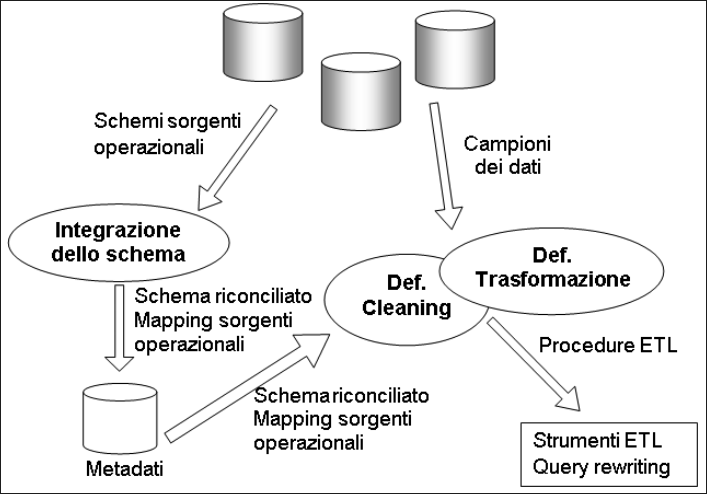
\includegraphics[width=.6\textwidth]{assets/integr-db-def.png}
\end{cimage}
%
\section{I Passi dell'Integrazione}\label{sec:db_i_passi_dell_integrazione} % (fold)
Analizzando più in dettaglio la fase di integrazione si evidenziano le seguenti operazioni:
\begin{itemize}
    \item \textbf{Analisi e normalizzazione}: consiste nell'analizzare i diversi schemi locali producendo come risultato un insieme di schemi concettuali localmente completi e consistenti;
    \item \textbf{Definizione dello schema riconciliato}: è la fase più importante in cui i diversi schemi locali vengono fusi in un unico schema globalmente consistente;
    \item \textbf{Definizione del mapping}: utilizzando lo schema logico riconciliato si definisce la relazione (\textbf{mapping}) tra concetti degli schemi sorgenti e dello schema riconciliato;
\end{itemize}
\begin{cimage}
    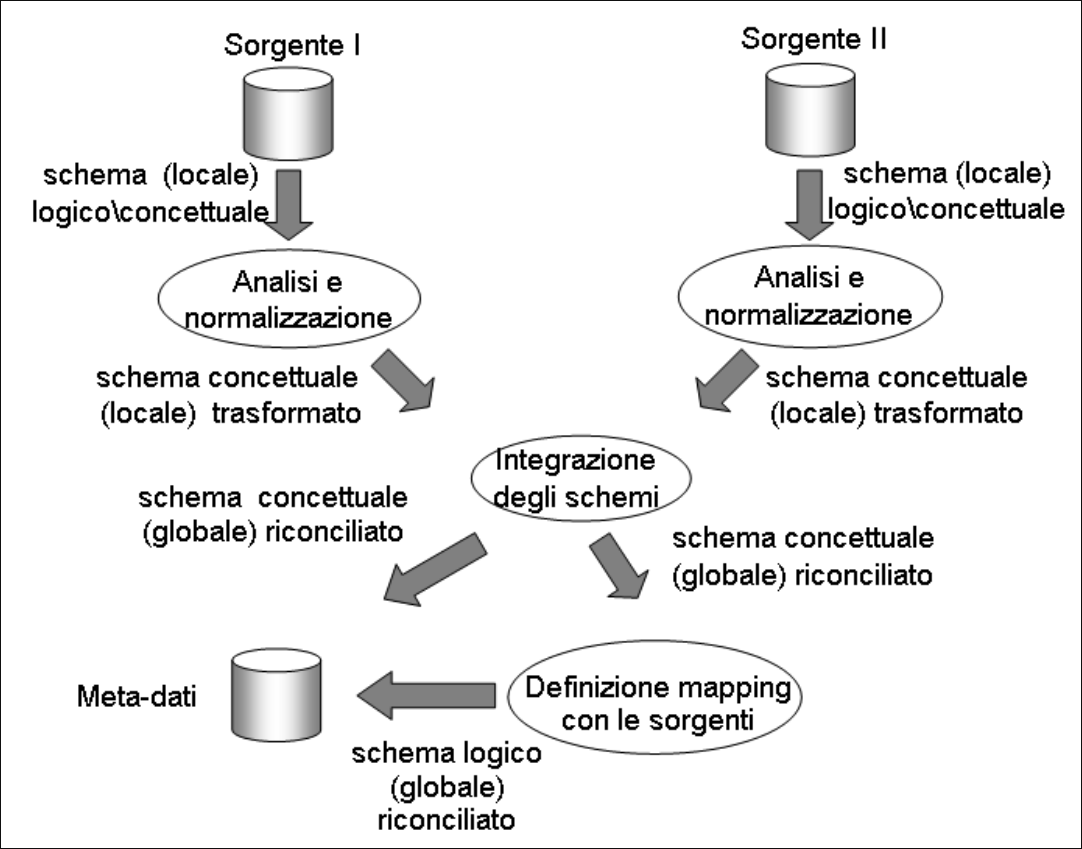
\includegraphics[width=.6\textwidth]{assets/passi-integrazoine-visual.png}
\end{cimage}
%
\subsection{Architettura per il SI integrato}\label{sub:architettura_per_il_si_integrato} % (fold)
La presenza di un livello di dati integrato modifica l'architettura del SI.
Le applicazioni operano su \textbf{viste} dello schema integrato che può essere:
\begin{description}
    \item[Virtuale] Viene definita solo la meta conoscenza necessaria a ottenere le informazioni sullo schema globale.
        Queste saranno create solo quando richieste mediante interrogazioni eseguite sugli schemi locali.
        Questa soluzione è quella maggiormente utilizzata.
    \item[Materializzato] I dati vengono trasformati e memorizzati in versione duplicata.
        Questa soluzione viene utilizzata per esempio nei sistemi DW.
\end{description}
A causa della complessità dell'operazione non è sempre possibile ottenere un unico schema globale; talvolta può essere sufficiente creare poche porzioni integrate a partire da molti schemi locali.
% subsection Architettura per il SI integrato (end)
%
\subsection{Analisi e Normalizzazione}\label{sub:db_analisi_e_normalizzazione} % (fold)
Durante la fase di analisi il progettista, confrontandosi con gli esperti del dominio applicativo, deve verificare la completezza degli schemi locali, sforzandosi di individuare eventuali correlazioni involontariamente omesse:
\begin{itemize}
    \item esplicitazione di dipendenze funzionali precedentemente tralasciate;
    \item individuazione di nuove associazioni tra le entità;
\end{itemize}
\begin{warning}
    Le trasformazioni apportate allo schema non devono però introdurre nuovi concetti, assenti nei dati presenti sulle sorgenti, bensì esplicitare tutti quelli ricavabili dai dati memorizzati nelle sorgenti operazionali
\end{warning}
Lo schema concettuale delle sorgenti rappresenta senz'altro il risultato principale dell'analisi, e deve essere espresso mediante lo stesso formalismo per tutte le sorgenti.
Dove assente esso deve essere ricavato per \textbf{reverse engineering}.
% subsection Analisi e Normalizzazione (end)
%
\subsection{Problemi da Affrontare}\label{sub:db_problemi_da_affrontare} % (fold)
Se le diverse sorgenti dati modellassero porzioni indipendenti e distinte nel mondo reale, il problema dell'integrazione non sussisterebbe.
Ciò non può avvenire in pratica poiché ogni azienda è un universo coeso in cui le diverse unità organizzative partecipano a processi comuni che condividono tutti o parte degli attori.
\emptyln{}
La fase di integrazione \textbf{non si deve limitare a evidenziare} le differenze di rappresentazione dei concetti comuni a più schermi, ma deve anche \textbf{identificare} l'insieme di concetti distinti e memorizzati in schemi differenti che sono correlati attraverso proprietà \red{semantiche}, chiamate \textbf{proprietà inter-schema}.
\emptyln{}
Le diversità nelle rappresentazioni dei concetti comuni sono causate da:
\begin{description}
    \item[Diversità di Prospettiva] Il punto di vista rispetto al quale \textbf{diversi gruppi di utenti} vedono uno stesso oggetto del dominio applicativo può differenziarsi notevolmente in base agli \textbf{aspetti rilevanti ai fini della funzione} a cui essi sono preposti.
        \begin{cimage}
            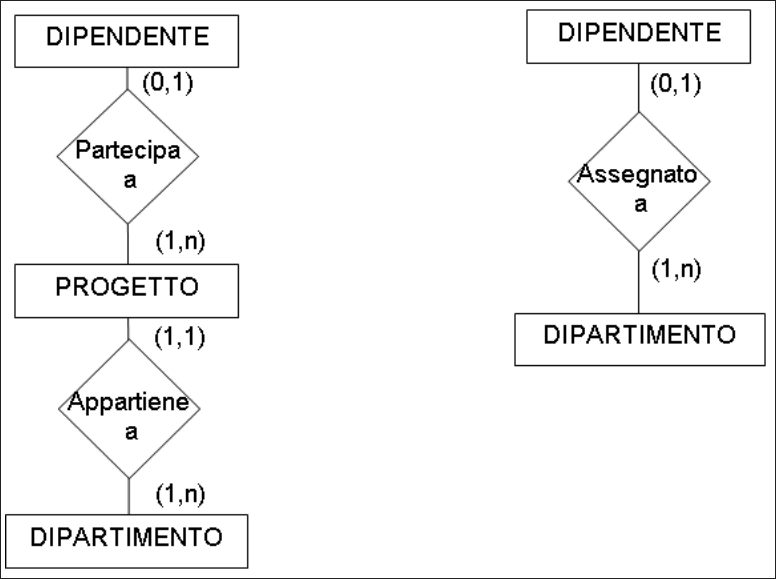
\includegraphics[width=.4\textwidth]{assets/div-prosp-schema.png}
            \caption{Nello schema a destra non è rilevante la distribuzione dei dipartimenti}\label{fig:div-prosp-schema}
        \end{cimage}
    \item[Equivalenza dei Costrutti del Modello] I formalismi di modellazione permettono di \textbf{rappresentare uno stesso concetto} utilizzando combinazioni diverse dei costrutti a disposizione.
        La diversità è puramente di tipo sintattico: le due modellazioni sono perfettamente equivalenti.
        \begin{cimage}
            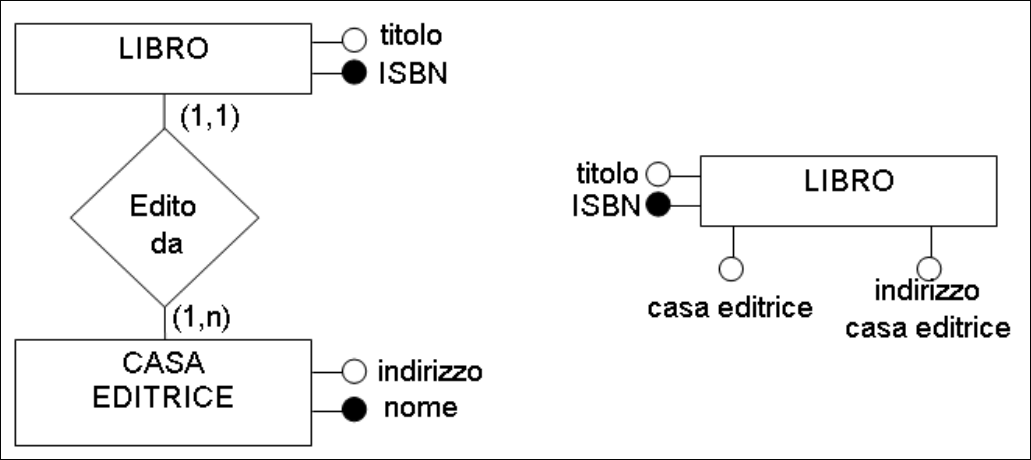
\includegraphics[width=.6\textwidth]{assets/equiv-costrutti-model-schema.png}
        \end{cimage}
        \begin{definition}{Schemi Equivalenti}{schemes-equiv}
            Due schemi $R_1$ e $R_2$ sono \textbf{equivalenti} se le loro istanze possono essere messe in corrispondenza uno-a-uno.
            \\
            L'equivalenza tra schemi implica che a livello estensionale esistono sempre due insiemi di dati, diversi ma equivalenti, che memorizzano le stesse informazioni.
            \begin{center}
                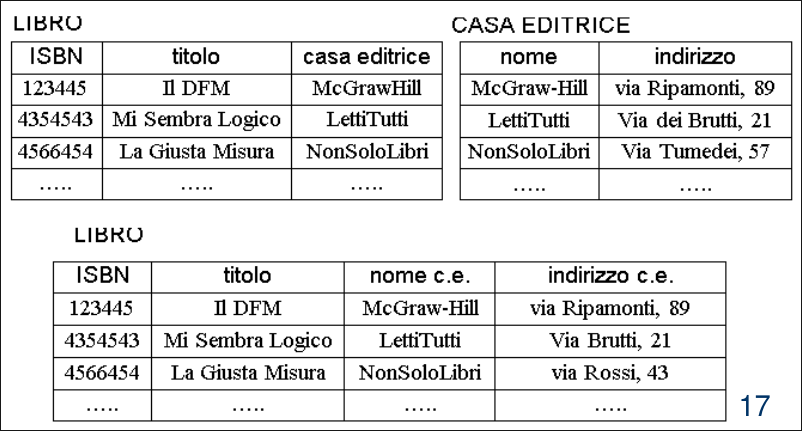
\includegraphics[width=.8\textwidth]{assets/dim-schem-equiv-table.png}
            \end{center}
        \end{definition}
    \item[Incompatibilità delle specifiche] Si verifica quando due schemi \textbf{modellano una stessa porzione del dominio applicativo e racchiudono concetti diversi}, in contrasto tra loro.
        Tale \red{diversità} deriva normalmente da \red{errate scelte progettuali} che possono coinvolgere per esempio la scelta dei nomi, dei tipi di dati e dei vincoli di integrità.
        \begin{cimage}
            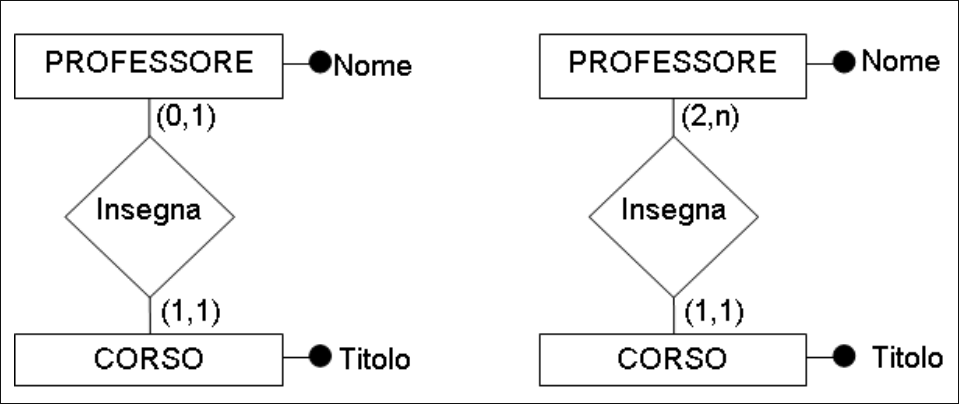
\includegraphics[width=.6\textwidth]{assets/incomp-spec-schema.png}
            \caption{Due schemi incompatibili}\label{fig:incomp-spec-schema}
        \end{cimage}
\end{description}
% subsection Problemi da Affrontare (end)
%
\subsection{Concetti Comuni}\label{sub:db_concetti_comuni} % (fold)
È necessario definire il tipo di relazione semantica esistente tra \textbf{concetti comuni} modellati diversamente in schemi distinti.
Quattro sono le possibili relazioni esistenti tra due distinte rappresentazioni $R_1$ e $R_2$ di uno stesso concetto:
\begin{itemize}
    \item \textbf{Identità}: vengono utilizzati gli stessi costrutti, il concetto è modellato dallo stesso punto di vista e non vengono commessi errori di specifica; in altre parole quando $R_1$ e $R_2$ coincidono;
    \item \textbf{Equivalenza}: $R_1$ e $R_2$ non sono esattamente le stesse poiché sono stati utilizzati costrutti diversi, ma equivalenti, e non sussistono errori di specifica o diversità di percezione;
    \item \textbf{Compatibilità}: $R_1$ e $R_2$ non sono né identici né equivalenti, ma i costrutti utilizzati e i punti di vista dei progettisti non sono in contrasto tra loro;
    \item \textbf{Incompatibilità}: $R_1$ e $R_2$ sono in \textbf{conflitto} a causa dell'incoerenza nelle specifiche.
        In altre parole la realtà modellata da $R_1$ nega la realtà modellata da $R_2$;
\end{itemize}
\begin{warning}
    A esclusione della situazione di \textbf{identità}, i casi precedenti determinano dei conflitti la cui soluzione rappresenta la componente principale nella fase di integrazione
\end{warning}
\begin{definition}{Conflitto}{}
    Si verifica un \textbf{conflitto} tra due rappresentazioni $R_1$ e $R_2$ di uno stesso concetto ogniqualvolta le due rappresentazioni non sono identiche.
\end{definition}
% subsection Concetti Comuni (end)
%
\subsection{Concetti Correlati}\label{sub:db_concetti_correlati} % (fold)
A seguito dell'integrazione, molti concetti diversi ma \textbf{correlati} verranno a trovarsi nello stesso schema dando vita a nuove relazioni che non erano percepibili in precedenza.
Tali relazioni sono dette \textbf{proprietà inter-schema} e devono essere identificate e rappresentate esplicitamente.
% subsection Concetti Correlati (end)
% section I Passi dell'Integrazione (end)
%
\section{Le Fasi dell'Integrazione}\label{sec:db_le_fasi_dell_integrazione} % (fold)
Risolvere i problemi fin qui elencati ed evidenziare le proprietà che emergono a seguito dell'integrazione degli schemi locali richiede un \textbf{complesso insieme di operazioni}, per la cui corretta gestione è necessario adottare una metodologia.
Le diverse metodologie proposte in letteratura concordano sulla \textbf{sequenza di passi} che devono essere \textbf{svolti} e che possono essere così sintetizzati:
\begin{itemize}
    \item \textbf{Preintegrazione}: comprende la fase di analisi e di scelta della strategia di integrazione;
    \item \textbf{Comparazione degli schemi}: durante questa fase gli \textbf{schemi locali} vengono confrontati per evidenziare i conflitti e i concetti correlati;
    \item \textbf{Allineamento degli schemi}: durante questa fase il progettista deve risolvere i conflitti precedentemente individuati;
    \item \textbf{Fusione e ristrutturazione degli schemi}: gli schemi resi coerenti possono essere fusi per creare un unico \textbf{schema globale};
\end{itemize}
% section Le Fasi dell'Integrazione (end)
%
\section{Strategie d'Integrazione}\label{sec:db_strategie_d_integrazione} % (fold)
Indicano \textbf{l'ordine} con cui si procederà all'integrazione degli schemi:
\begin{itemize}
    \item \textbf{tecniche ennarie}: il processo di integrazione considera più di due schemi contemporaneamente.
        Ogni concetto viene analizzato avendo a disposizione contemporaneamente tutte le informazioni che lo caratterizzano.
        Inoltre si diminuisce il numero totale di comparazioni tra concetti poiché ognuno di essi viene analizzato una volta sola.
    \item \textbf{tecniche binarie}: il processo di integrazione considera sempre coppie di schemi, rendendo ogni passo di integrazione più semplice grazie al ridotto numero di concetti coinvolti contemporaneamente.
        Sono dette \textbf{a scala} quando i nuovi schemi sono integrati allo schema temporaneo \textbf{determinato} fino a quel momento; in questo modo è possibile definire l'ordine con cui i diversi schemi sorgenti andranno esaminati e aggiungi allo schema riconciliato.
        \begin{tip}
            Normalmente si preferisce iniziare dalle sorgenti che costituiscono il \textbf{cuore} del sistema informativo e la cui integrazione definirà lo scheletro dello schema riconciliato
        \end{tip}
\end{itemize}
\begin{cimage}
    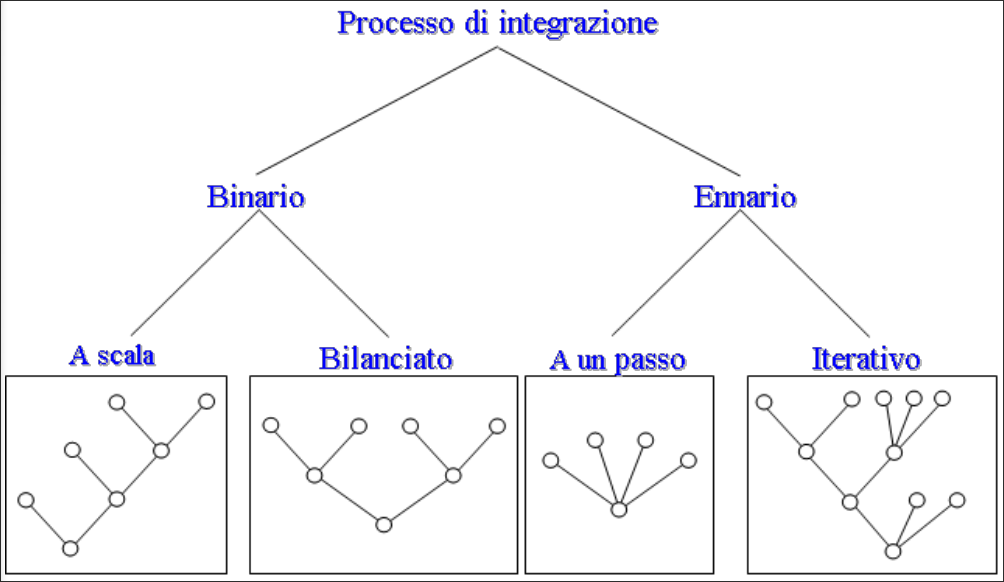
\includegraphics[width=.6\textwidth]{assets/strat-int-graph.png}
\end{cimage}
% section Strategie d'Integrazione (end)
%
\section{Comparazione degli Schemi}\label{sec:db_comparazione_degli_schemi} % (fold)
Questa fase consiste in \textbf{un'analisi comparativa dei diversi schemi} che mira a \textbf{identificare} le correlazioni e conflitti tra i concetti in essi espressi.
La sua efficacia dipende dalle conoscenze acquisite dal progettista rispetto al dominio applicativo e alla struttura delle sorgenti informative.
\\
I conflitti che possono essere evidenziati appartengono a 4 categorie:
\begin{itemize}
    \item \textbf{conflitti di eterogeneità}: indicano discrepanze dovute all'utilizzo di formalismi con diverso potere espressivo negli schemi sorgenti;
    \item \textbf{conflitti sui nomi}: si verificano a causa delle differenze nelle terminologie utilizzate nei diversi schemi sorgenti:
        \begin{itemize}
            \item \textbf{Omonimie}: lo stesso termine viene utilizzato per denotare due concetti diversi;
            \item \textbf{Sinonimie}: due nomi diversi denotano uno stesso concetto;
        \end{itemize}
\end{itemize}
\begin{warning}
    Mentre le \textbf{omonimie} possono essere individuate da una semplice \textbf{comparazione dei concetti} che presentano gli stessi nomi in schemi diversi, per riconoscere eventuali \textbf{sinonimi} è necessaria una conoscenza approfondita del dominio applicativo
\end{warning}
%
\subsection{Conflitti Semantici}\label{sub:db_conflitti_semantici} % (fold)
I \textbf{conflitti semantici} si verificano quando due schemi sorgenti modellano la stessa porzione di mondo reale a un diverso livello di astrazione e dettaglio.
\begin{note}
    Il \red{livello di dettaglio} adottato negli schemi locali è \textbf{diverso} e di conseguenza anche l'insieme di informazioni rappresentabili cambia
\end{note}
\begin{cimage}
    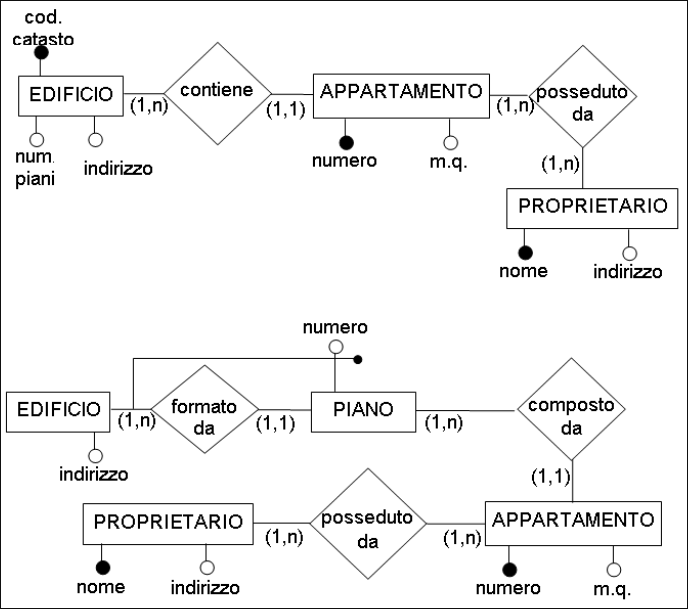
\includegraphics[width=.6\textwidth]{assets/comp-schem-visual.png}
\end{cimage}
% subsection Conflitti Semantici (end)
%
\subsection{Conflitti Strutturali}\label{sub:db_conflitti_strutturali} % (fold)
I \textbf{conflitti strutturali} sono causati da scelte diverse nella modellazione di uno stesso concetto, oppure dall'applicazione di differenti vincoli di integrità.
\\
Possono essere classificati in quattro categorie:
\begin{itemize}
    \item \textbf{conflitti di tipo}, si verificano quando uno stesso concetto è modellato utilizzando due costrutti diversi;
    \item \textbf{conflitti di dipendenza}, si verificano quando due o più concetti sono correlati con dipendenze diverse in schemi diversi;
    \item \textbf{conflitti di chiave}, si verificano quando per uno stesso concetto vengono utilizzati identificatori diversi in schemi diversi;
    \item \textbf{conflitti di comportamento}, si verificano quando diverse politiche di cancellazione/modifica dei dati vengono adottate per uno stesso concetto in schemi diversi;
\end{itemize}
% subsection Conflitti Strutturali (end)
% section Comparazione degli Schemi (end)
% chapter Integrazione di Basi di Dati (end)
